\chapter{Hiện thực hệ thống}
\section{Các tính năng chính}
\textbf{API} cung cấp các tính năng chính sau:
\begin{itemize}
    \item \textbf{Đăng ký và đăng nhập người dùng}: 
    \begin{itemize}
        \item Endpoint \texttt{/api/register/}: Cho phép người dùng tạo tài khoản mới với thông tin như email và mật khẩu.
        \item Endpoint \texttt{/api/login/}: Xác thực thông tin người dùng và trả về token để quản lý phiên đăng nhập.
    \end{itemize}
    \item \textbf{Xác thực và phân quyền người dùng}: 
    \begin{itemize}
        \item Đảm bảo chỉ những người dùng được phép mới có thể truy cập các tài nguyên cụ thể thông qua token xác thực.
    \end{itemize}
    \item \textbf{Quản lý thông tin người dùng (CRUD)}: 
    \begin{itemize}
        \item Endpoint \texttt{/api/users/}: Cho phép thêm, sửa, xóa và xem thông tin người dùng.
    \end{itemize}
    \item \textbf{Gửi email xác minh tài khoản}: 
    \begin{itemize}
        \item Endpoint \texttt{/api/verify-email/}: Gửi email xác minh để kích hoạt tài khoản người dùng.
    \end{itemize}
    \item \textbf{Quản lý nhạc và video âm nhạc}:
    \begin{itemize}
        \item Endpoint \texttt{/api/songs/}: Hiển thị danh sách bài hát.
        \item Endpoint \texttt{/api/songs/<id>/}: Hiển thị chi tiết bài hát.
        \item Endpoint \texttt{/api/songs/}: Cho phép thêm bài hát mới (POST).
        \item Endpoint \texttt{/api/songs/<id>/}: Chỉnh sửa bài hát (PUT/PATCH).
        \item Endpoint \texttt{/api/songs/<id>/}: Xóa bài hát (DELETE).
        \item Endpoint \texttt{/api/songs/search/}: Tìm kiếm bài hát theo tên, nghệ sĩ hoặc thể loại.
        \item Endpoint \texttt{/api/videos/}: Quản lý video âm nhạc (tương tự như bài hát).
    \end{itemize}
    \item \textbf{Quản lý danh sách phát và album}:
    \begin{itemize}
        \item Endpoint \texttt{/api/playlists/}: Quản lý danh sách phát nhạc của người dùng.
        \item Endpoint \texttt{/api/albums/}: Cho phép người dùng tạo album nhạc cá nhân.
    \end{itemize}
    \item \textbf{Quản lý yêu thích}:
    \begin{itemize}
        \item Endpoint \texttt{/api/favorites/}: Quản lý danh sách bài hát yêu thích của người dùng.
    \end{itemize}
\end{itemize}

\textbf{Frontend} cung cấp các tính năng chính sau:
\begin{itemize}
    \item \textbf{Giao diện đăng ký và đăng nhập}:
    \begin{itemize}
        \item Người dùng có thể đăng ký tài khoản mới hoặc đăng nhập vào hệ thống thông qua giao diện thân thiện.
    \end{itemize}
    \item \textbf{Giao diện phát nhạc trực tuyến}:
    \begin{itemize}
        \item Tích hợp trình phát nhạc, cho phép người dùng nghe nhạc trực tuyến.
        \item Hỗ trợ phát video âm nhạc.
    \end{itemize}
    \item \textbf{Giao diện quản lý danh sách phát nhạc và album}:
    \begin{itemize}
        \item Người dùng có thể tạo, chỉnh sửa, xóa danh sách phát và album cá nhân.
    \end{itemize}
    \item \textbf{Giao diện quản lý yêu thích}:
    \begin{itemize}
        \item Hiển thị danh sách bài hát yêu thích của người dùng.
    \end{itemize}
    \item \textbf{Trang Admin}:
    \begin{itemize}
        \item Quản trị viên có thể quản lý người dùng, bài hát, video, và thể loại nhạc thông qua giao diện quản trị.
    \end{itemize}
    \item \textbf{Tìm kiếm và khám phá}:
    \begin{itemize}
        \item Người dùng có thể tìm kiếm bài hát, nghệ sĩ, hoặc thể loại nhạc thông qua giao diện tìm kiếm.
    \end{itemize}
    \item \textbf{Tính năng chat (Optional)}:
    \begin{itemize}
        \item Tích hợp tính năng chat trong giao diện web để người dùng có thể tương tác với nhau.
    \end{itemize}
    \begin{figure}[h]
    \centering
    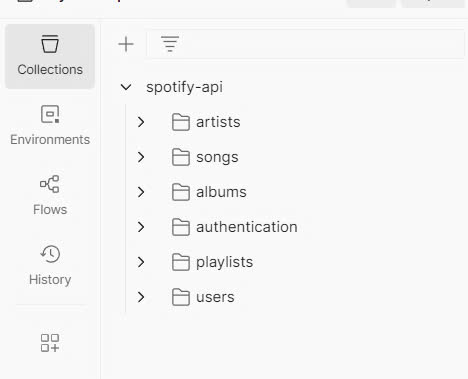
\includegraphics[width=1\textwidth]{imgs/api-postman.jpg}
    \caption{API trên Postman}
\end{figure}
\end{itemize}

\section{Giao diện và hình ảnh minh họa}

\subsection{Quản lý nhạc}

\subsubsection{Hiển thị danh sách}
API cung cấp endpoint \texttt{/api/songs/} để lấy danh sách các bài hát trong hệ thống. Frontend hiển thị danh sách này với các thông tin cơ bản như tên bài hát, nghệ sĩ, và thể loại để người dùng có thể dễ dàng duyệt qua.

\begin{figure}[H]
    \centering
    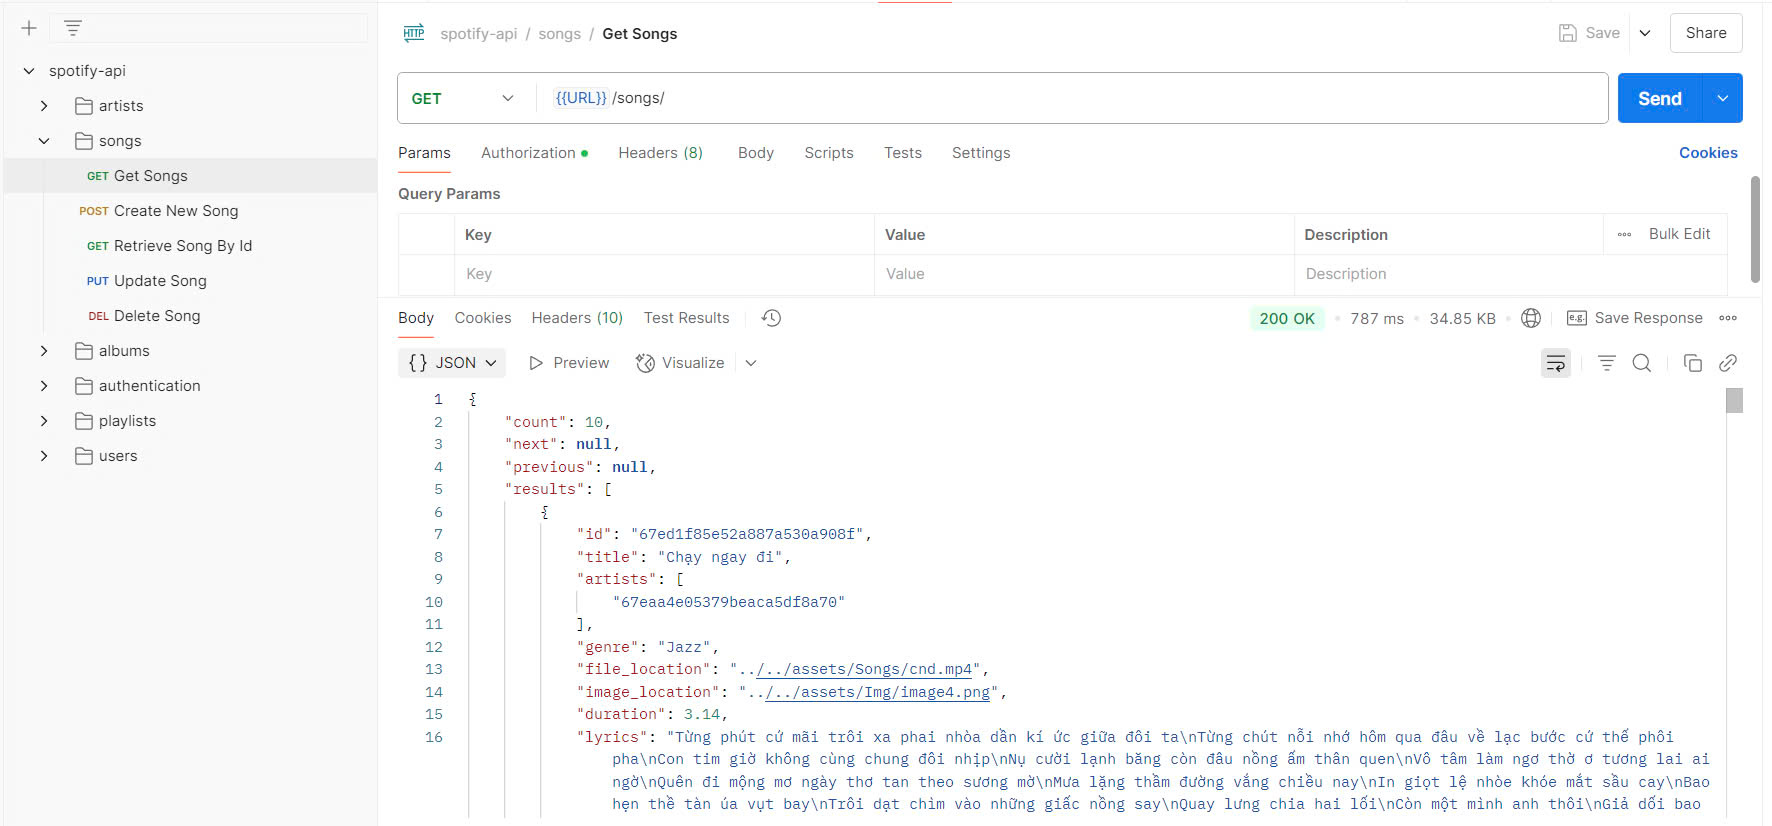
\includegraphics[width=1\textwidth]{imgs/api-songs.jpg}
    \caption{API lấy danh sách bài hát (Postman)}
\end{figure}

\begin{figure}[H]
    \centering
    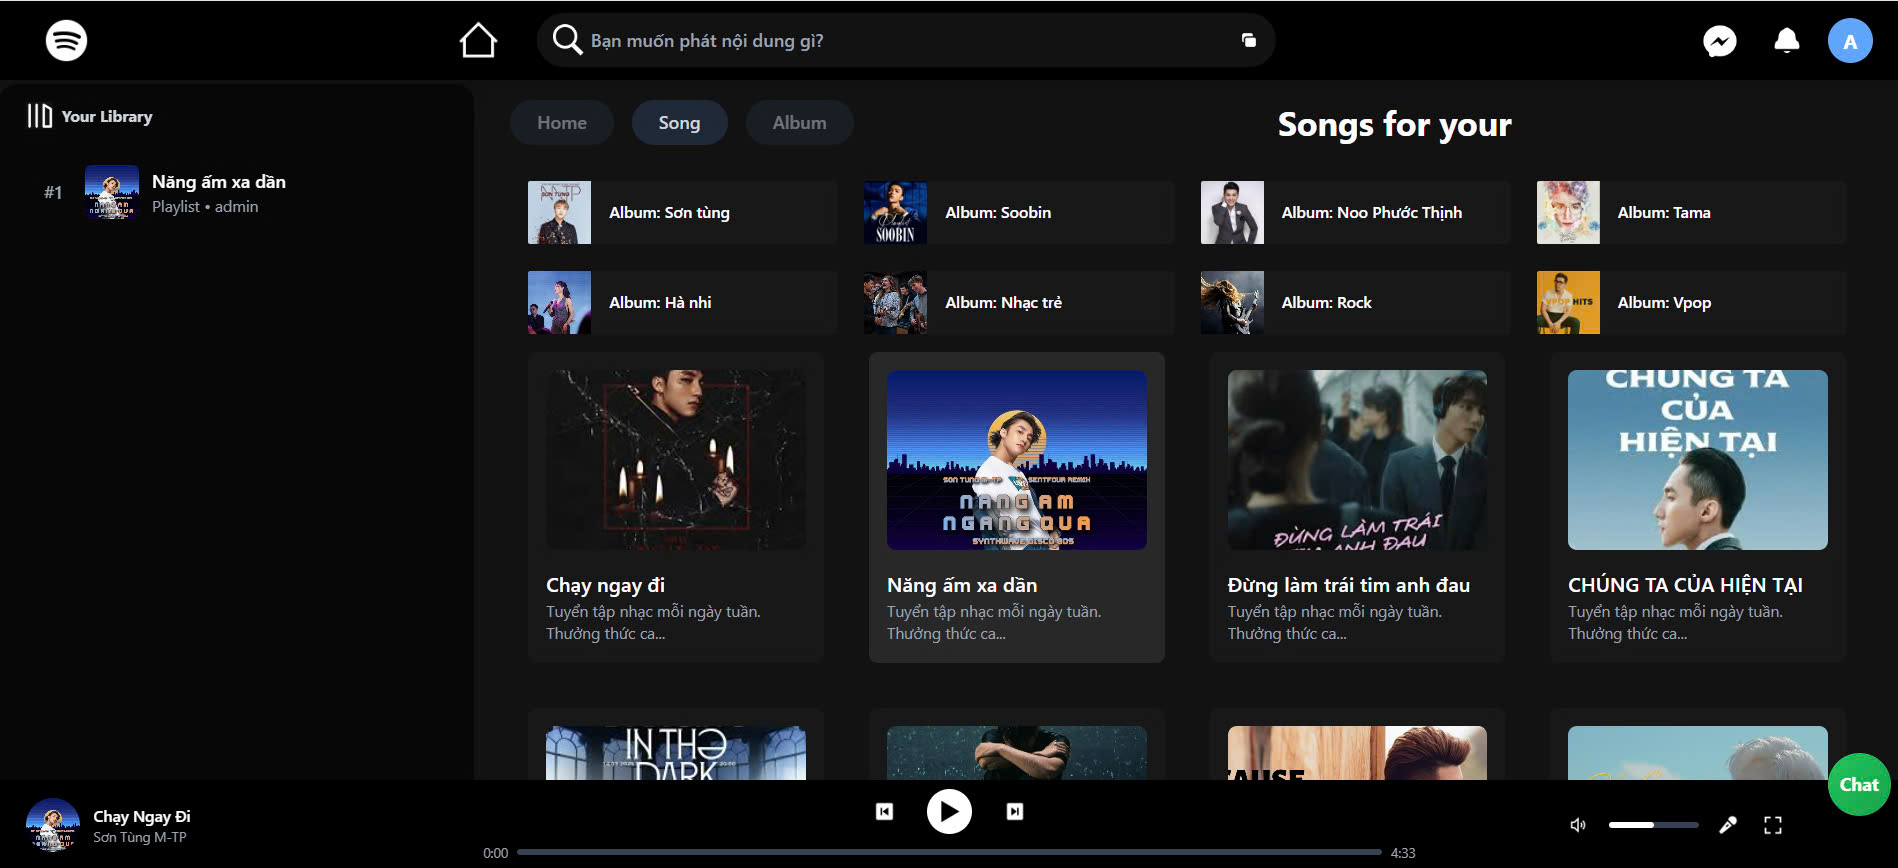
\includegraphics[width=1\textwidth]{imgs/frontend-songs.jpg}
    \caption{Giao diện danh sách bài hát (Frontend)}
\end{figure}
\begin{figure}[H]
    \centering
    \includegraphics[width=1\textwidth]{imgs/frontend-admin-songs.jpg}
    \caption{Giao diện danh sách bài hát trên admin}
\end{figure}

\subsubsection{Hiển thị chi tiết bài hát}
Người dùng có thể xem chi tiết bài hát thông qua endpoint \texttt{/api/songs/<id>/}. Endpoint này trả về các thông tin chi tiết của bài hát như tên bài hát, nghệ sĩ, album, thời gian phát, và lời bài hát.

\begin{figure}[H]
    \centering
    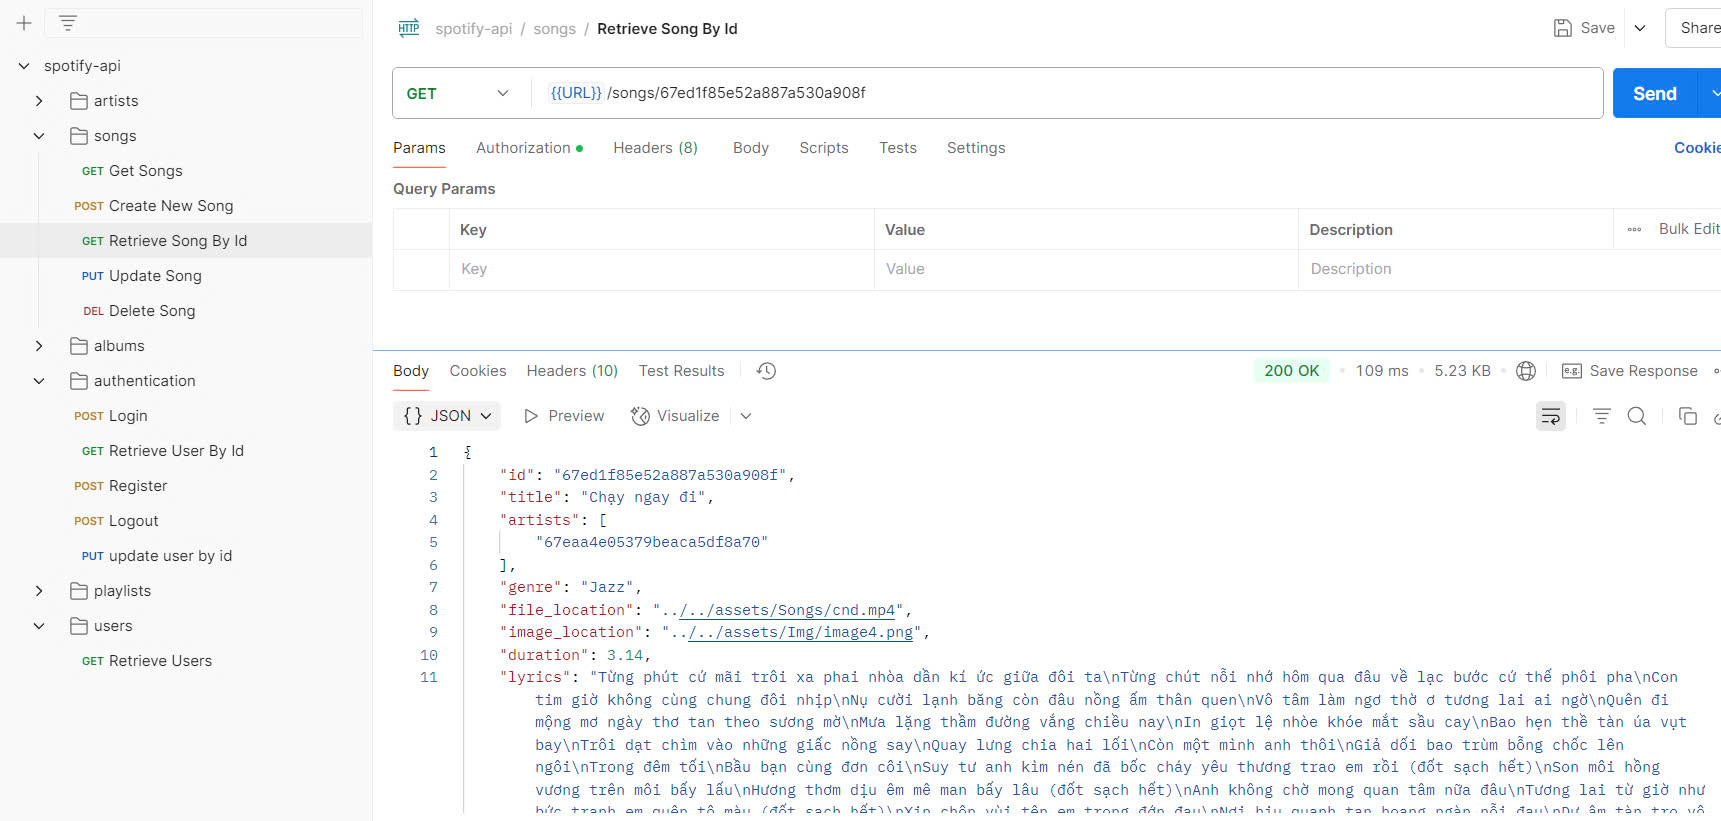
\includegraphics[width=1\textwidth]{imgs/api-song-detail.jpg}
    \caption{API chi tiết bài hát (Postman)}
\end{figure}

\begin{figure}[H]
    \centering
    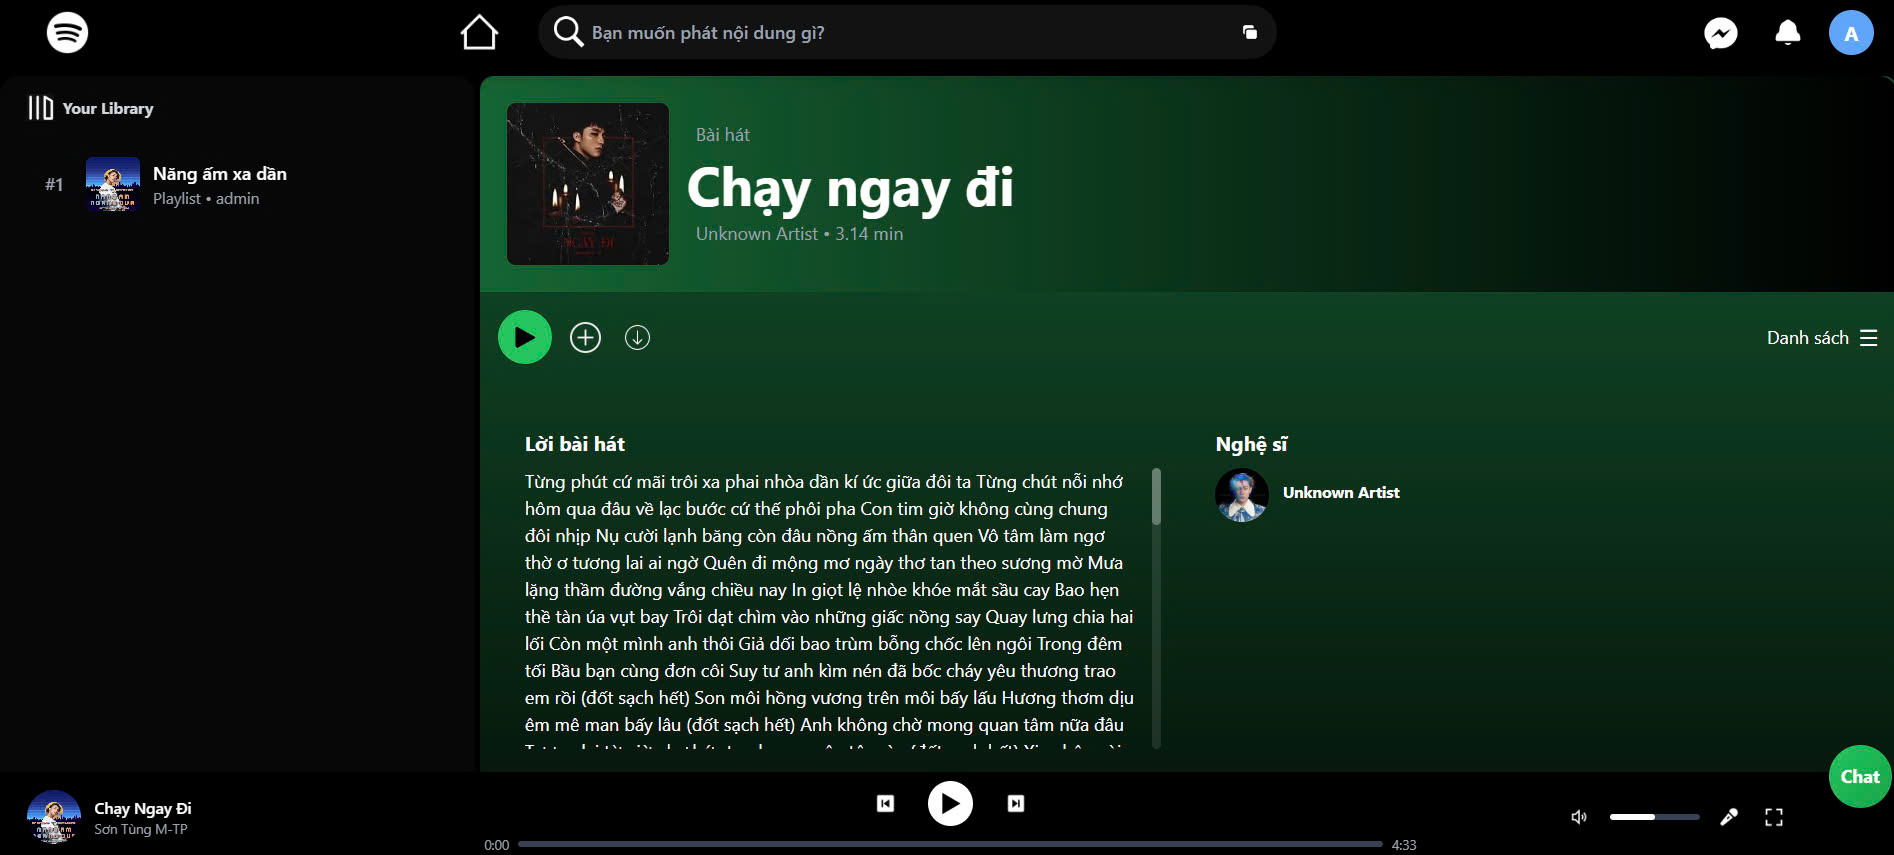
\includegraphics[width=1\textwidth]{imgs/frontend-song-detail.jpg}
    \caption{Giao diện chi tiết bài hát (Frontend)}
\end{figure}

\subsubsection{Nghe thử bài hát}
Frontend tích hợp trình phát nhạc, cho phép người dùng nghe thử bài hát trực tuyến thông qua URL phát nhạc được trả về từ API. Người dùng chỉ cần nhấn vào bài hát để bắt đầu nghe.

\begin{figure}[H]
    \centering
    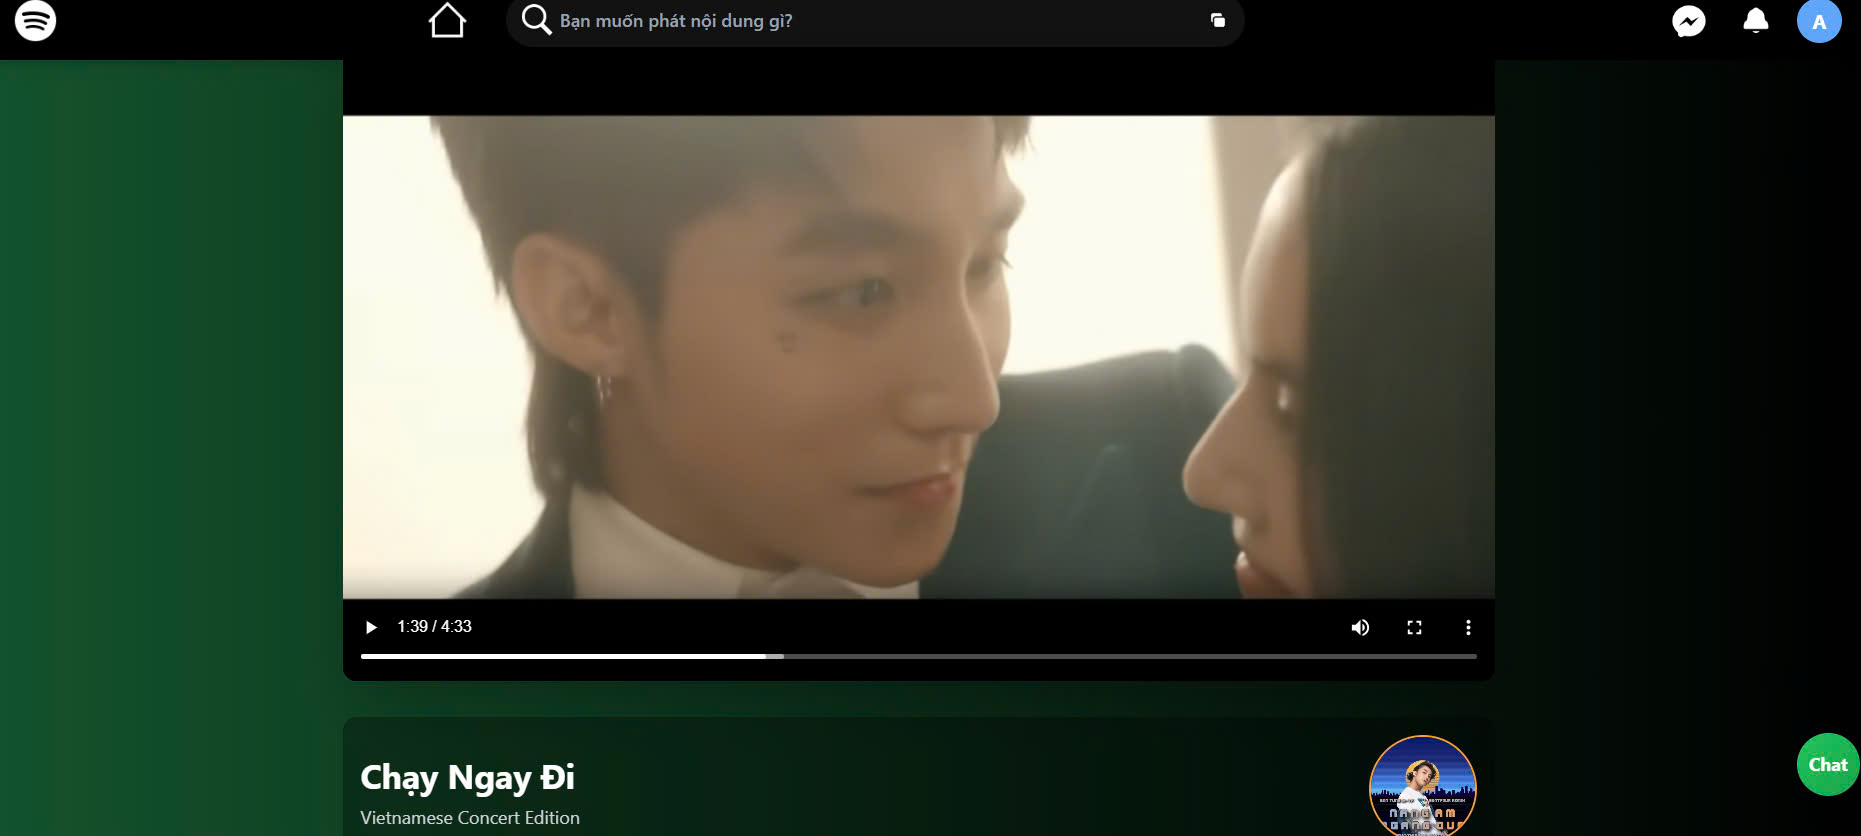
\includegraphics[width=1\textwidth]{imgs/frontend-player.jpg}
    \caption{Giao diện trình phát nhạc}
\end{figure}

\subsubsection{Thêm bài hát mới}
Quản trị viên có thể thêm bài hát mới vào hệ thống thông qua endpoint \texttt{/api/songs/} với phương thức POST. Dữ liệu cần thiết bao gồm tên bài hát, nghệ sĩ, thể loại, URL phát nhạc, và các thông tin liên quan khác.

\begin{figure}[H]
    \centering
    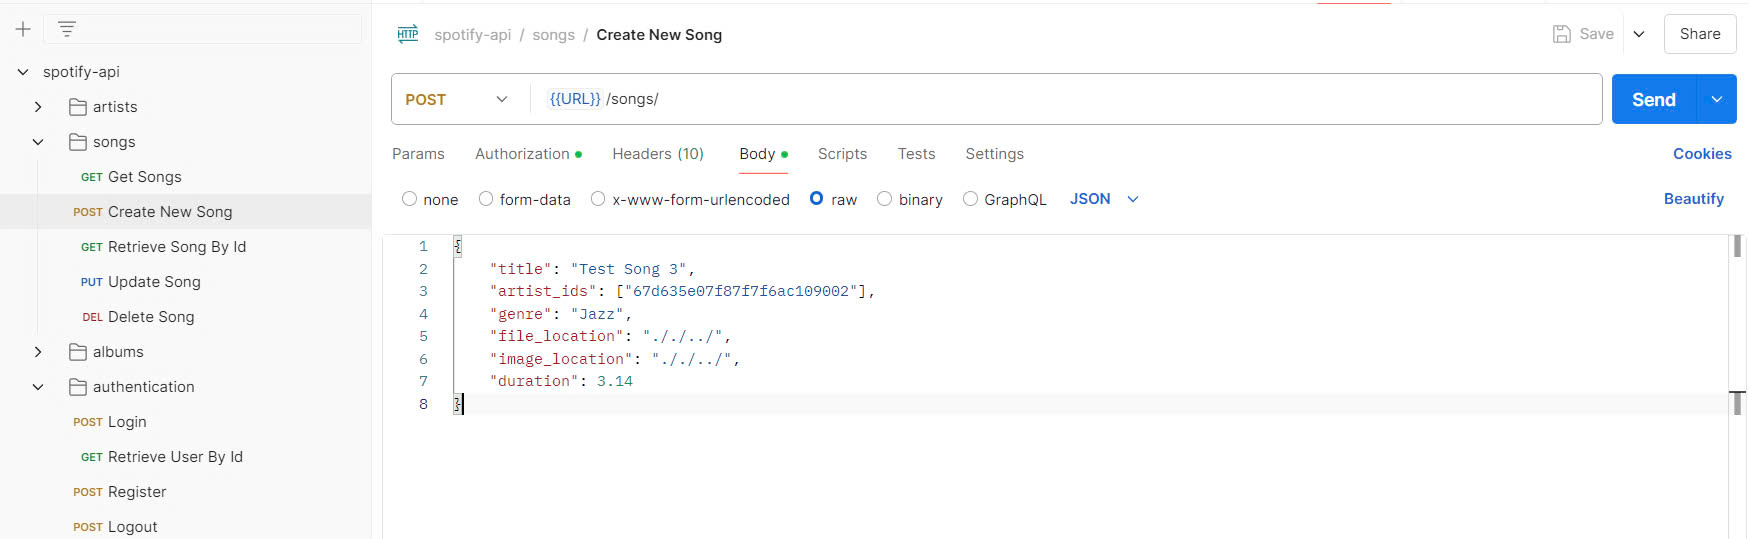
\includegraphics[width=1\textwidth]{imgs/api-add-song.jpg}
    \caption{API thêm bài hát (POST)}
\end{figure}

\begin{figure}[H]
    \centering
    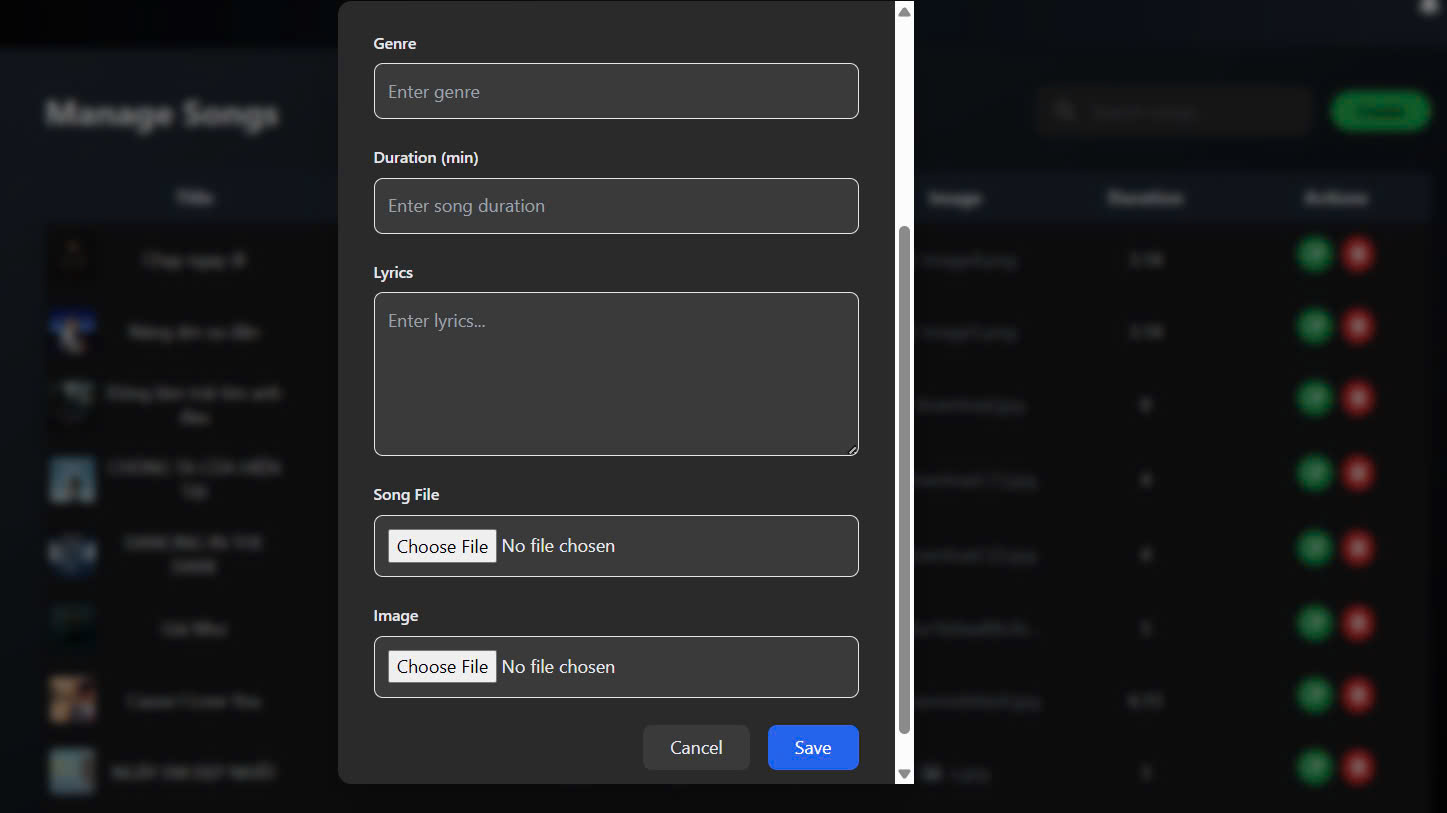
\includegraphics[width=1\textwidth]{imgs/frontend-add-song.jpg}
    \caption{Giao diện thêm bài hát}
\end{figure}

\subsubsection{Chỉnh sửa bài hát}
Quản trị viên có thể chỉnh sửa thông tin bài hát thông qua endpoint \texttt{/api/songs/<id>/} với phương thức PUT hoặc PATCH. Các thông tin có thể chỉnh sửa bao gồm tên bài hát, nghệ sĩ, thể loại, và URL phát nhạc.

\begin{figure}[H]
    \centering
    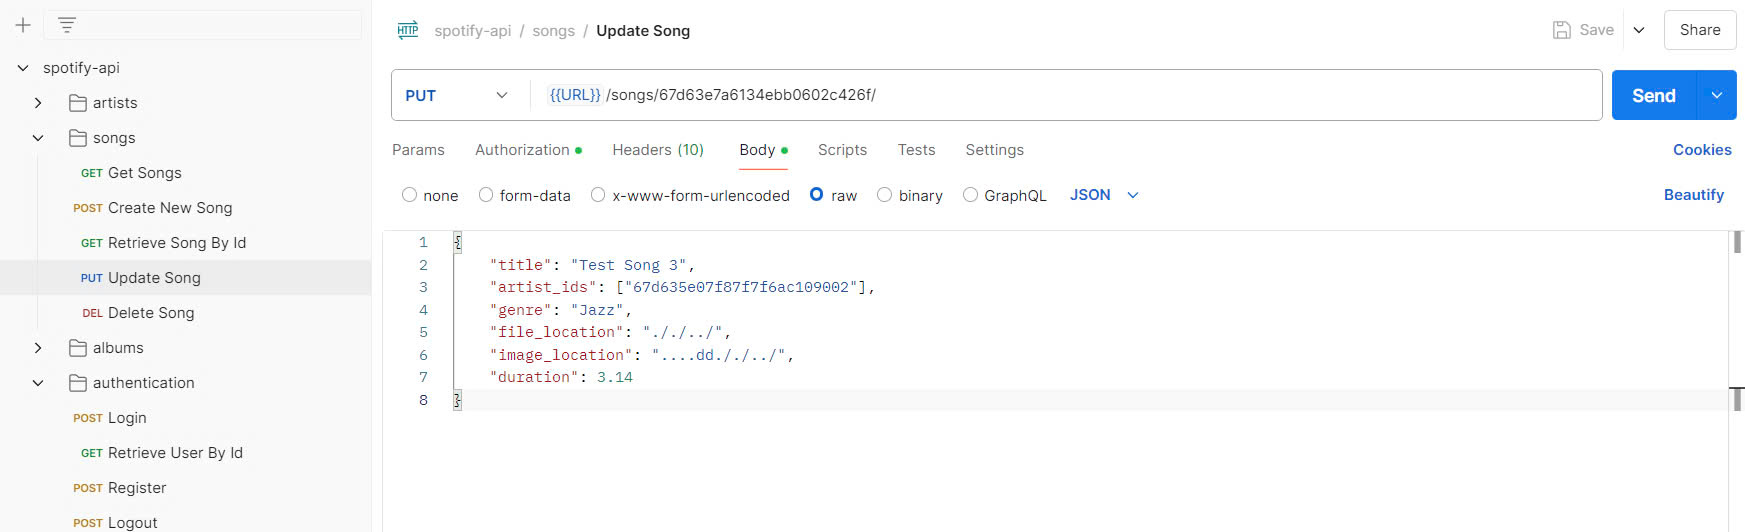
\includegraphics[width=1\textwidth]{imgs/api-edit-song.jpg}
    \caption{API chỉnh sửa bài hát (PUT)}
\end{figure}

\begin{figure}[H]
    \centering
    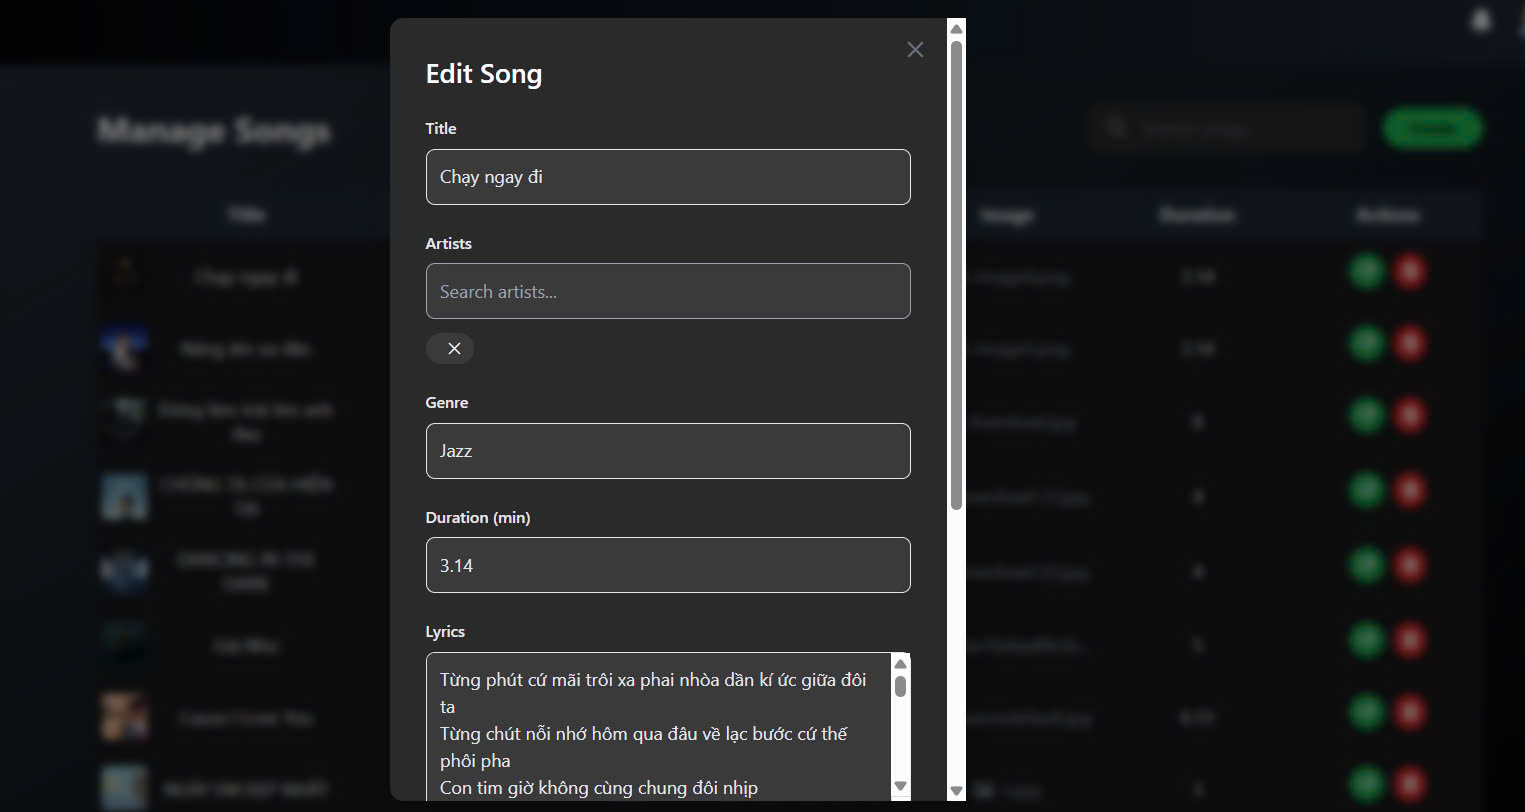
\includegraphics[width=1\textwidth]{imgs/frontend-edit-song.jpg}
    \caption{Giao diện chỉnh sửa bài hát}
\end{figure}

\subsubsection{Xóa nhạc}
Endpoint \texttt{/api/songs/<id>/} với phương thức DELETE cho phép quản trị viên xóa bài hát khỏi hệ thống khi không còn cần thiết. Khi nhấn vào icon delete thì bài hát được xóa và thông báo thành công

\begin{figure}[H]
    \centering
    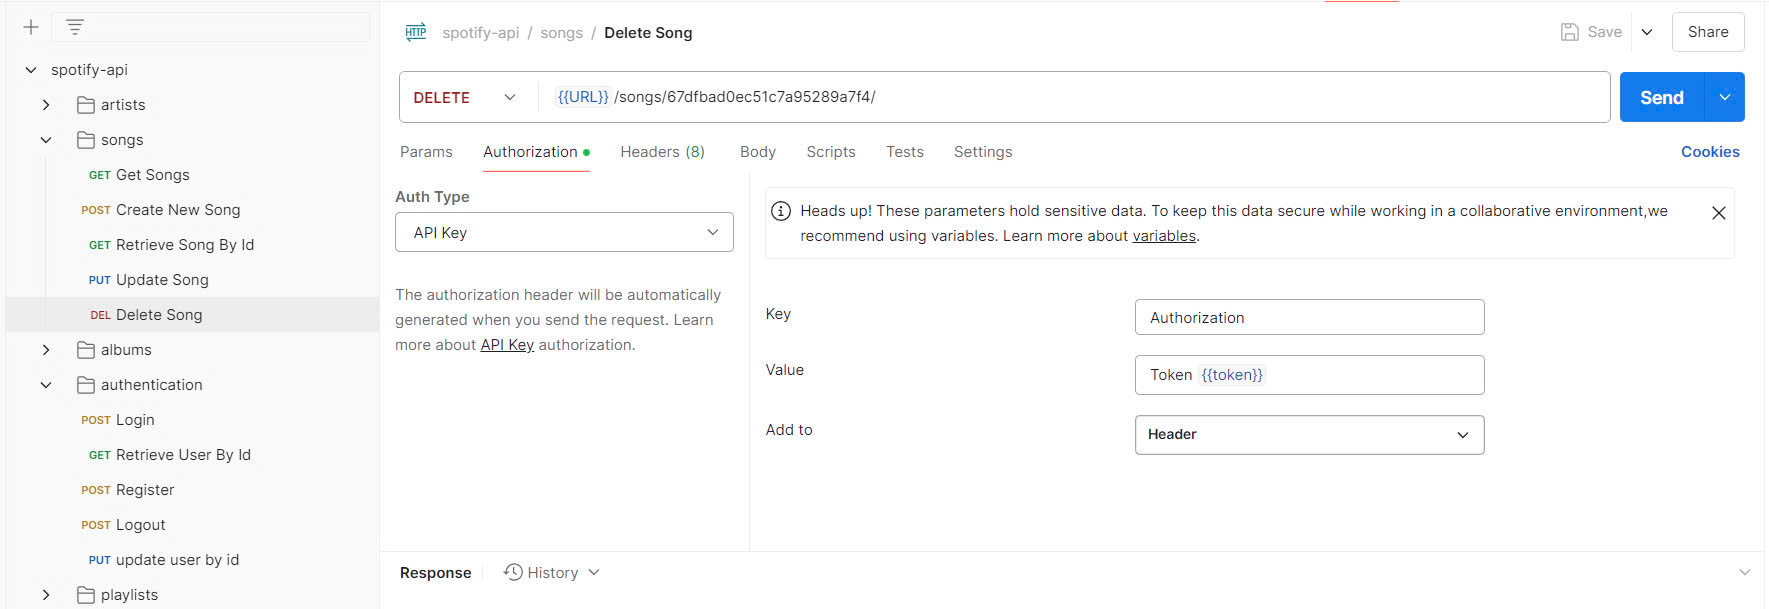
\includegraphics[width=1\textwidth]{imgs/api-delete-song.jpg}
    \caption{API xóa bài hát (DELETE)}
\end{figure}

\begin{figure}[H]
    \centering
    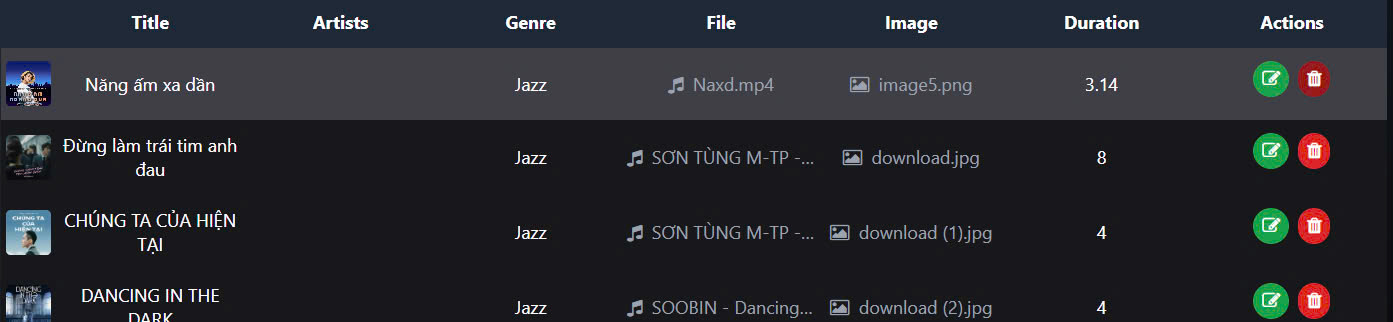
\includegraphics[width=1\textwidth]{imgs/frontend-delete-song.jpg}
    \caption{Giao diện xóa bài hát}
\end{figure}

\subsubsection{Tìm kiếm nhạc}
Hỗ trợ tìm kiếm bài hát qua endpoint, cho phép người dùng tìm kiếm bài hát theo các tiêu chí như tên bài hát, nghệ sĩ, hoặc thể loại.

\begin{figure}[H]
    \centering
    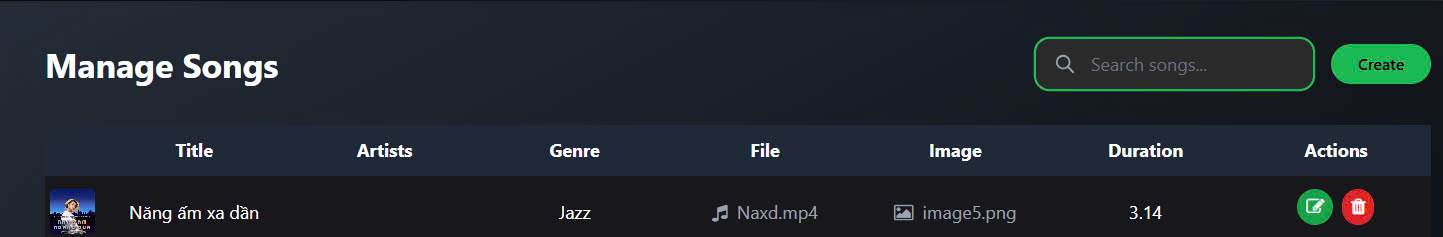
\includegraphics[width=1\textwidth]{imgs/frontend-search-song.jpg}
    \caption{Giao diện tìm kiếm bài hát}
\end{figure}

\section{Quản lý albums}
\subsection{Hiển thị danh sách}
Endpoint \texttt{/api/albums/} trả về danh sách các album có sẵn trong hệ thống. Frontend hiển thị danh sách này với các thông tin như tên album, ngày phát hành, nghệ sĩ liên quan, và ảnh đại diện.

\subsection{Hiển thị chi tiết album}
Người dùng có thể xem chi tiết về một album qua endpoint \texttt{/api/albums/<id>/}, bao gồm thông tin như tên album, ngày phát hành, danh sách bài hát, và nghệ sĩ liên quan.

\subsection{Thêm album}
Quản trị viên có thể thêm album mới vào hệ thống thông qua endpoint \texttt{/api/albums/} với phương thức POST. Dữ liệu cần thiết bao gồm:
\begin{itemize}
    \item \textbf{title}: Tên album.
    \item \textbf{release\_date}: Ngày phát hành.
    \item \textbf{album\_type}: Loại album (ví dụ: single, album đầy đủ).
    \item \textbf{artist\_ids}: Danh sách ID nghệ sĩ liên quan.
    \item \textbf{song\_ids}: Danh sách ID bài hát trong album.
    \item \textbf{image\_file}: Ảnh đại diện của album.
\end{itemize}

\subsection{Chỉnh sửa album}
Endpoint \texttt{/api/albums/<id>/} với phương thức PUT hoặc PATCH cho phép chỉnh sửa thông tin album, bao gồm tên, ngày phát hành, danh sách bài hát, và nghệ sĩ liên quan.

\subsection{Xóa album}
Quản trị viên có thể xóa album khỏi hệ thống qua endpoint \texttt{/api/albums/<id>/} với phương thức DELETE.

\section{Quản lý nghệ sĩ (artists)}
\subsection{Hiển thị danh sách}
Endpoint \texttt{/api/artists/} trả về danh sách các nghệ sĩ trong hệ thống. Frontend hiển thị danh sách này với các thông tin như tên nghệ sĩ, năm ra mắt, và ảnh đại diện.

\subsection{Hiển thị chi tiết nghệ sĩ}
Người dùng có thể xem chi tiết về một nghệ sĩ qua endpoint \texttt{/api/artists/<id>/}, bao gồm thông tin như tên, tiểu sử, năm ra mắt, và danh sách album hoặc bài hát liên quan.

\subsection{Thêm nghệ sĩ}
Quản trị viên có thể thêm nghệ sĩ mới vào hệ thống thông qua endpoint \texttt{/api/artists/} với phương thức POST. Dữ liệu cần thiết bao gồm:
\begin{itemize}
    \item \textbf{name}: Tên nghệ sĩ.
    \item \textbf{bio}: Tiểu sử.
    \item \textbf{debut\_year}: Năm ra mắt.
    \item \textbf{artist\_photo}: Ảnh đại diện của nghệ sĩ.
\end{itemize}

\subsection{Chỉnh sửa nghệ sĩ}
Endpoint \texttt{/api/artists/<id>/} với phương thức PUT hoặc PATCH cho phép chỉnh sửa thông tin nghệ sĩ, bao gồm tên, tiểu sử, năm ra mắt, và ảnh đại diện.

\subsection{Xóa nghệ sĩ}
Quản trị viên có thể xóa nghệ sĩ khỏi hệ thống qua endpoint \texttt{/api/artists/<id>/} với phương thức DELETE.

\section{Quản lý người dùng (users)}
\subsection{Hiển thị danh sách}
Endpoint \texttt{/api/users/} trả về danh sách tất cả người dùng trong hệ thống. Quản trị viên có thể sử dụng endpoint này để theo dõi và quản lý người dùng. Frontend hiển thị danh sách với các thông tin như tên người dùng, email, vai trò, và trạng thái tài khoản.

\subsection{Hiển thị chi tiết người dùng}
Quản trị viên có thể xem chi tiết thông tin của một người dùng qua endpoint \texttt{/api/users/<id>/}, bao gồm các thông tin như tên người dùng, email, vai trò, và các thông tin cá nhân khác.

\subsection{Thêm người dùng}
Quản trị viên có thể thêm người dùng mới vào hệ thống thông qua endpoint \texttt{/api/users/} với phương thức POST. Dữ liệu cần thiết bao gồm:
\begin{itemize}
    \item \textbf{username}: Tên đăng nhập.
    \item \textbf{email}: Địa chỉ email.
    \item \textbf{password}: Mật khẩu.
    \item \textbf{isstaff}: Vai trò (admin hoặc user).
     \item \textbf{issuperuser}: Quyền....
\end{itemize}

\subsection{Chỉnh sửa người dùng}
Endpoint \texttt{/api/users/<id>/} với phương thức PUT hoặc PATCH cho phép chỉnh sửa thông tin người dùng, bao gồm tên, email, và vai trò.

\subsection{Xóa người dùng}
Quản trị viên có thể xóa người dùng khỏi hệ thống qua endpoint \texttt{/api/users/<id>/} với phương thức DELETE.

\section{Quản lý server}
\subsection{Khởi động server}
Server có thể được khởi động bằng lệnh \texttt{python manage.py runserver}, sau khi môi trường đã được cấu hình và ứng dụng đã được cài đặt đầy đủ.

\subsection{Tắt server}
Để tắt server, người dùng chỉ cần dừng tiến trình đang chạy trong terminal bằng cách sử dụng lệnh \texttt{CTRL+C} hoặc tắt ứng dụng trực tiếp từ quản lý dịch vụ.

\section{Frontend Client}
\subsection{Đăng nhập}
Người dùng có thể đăng nhập vào hệ thống thông qua giao diện frontend. Thông tin đăng nhập sẽ được gửi đến endpoint \texttt{/api/login/} để xác thực và nhận token cho các yêu cầu tiếp theo.

\subsection{Đăng ký}
Người dùng có thể đăng ký tài khoản mới qua giao diện frontend. Các thông tin đăng ký được gửi đến endpoint \texttt{/api/register/} để tạo tài khoản mới trong hệ thống.

\subsection{Trang chủ}
Trang chủ hiển thị danh sách các bài hát nổi bật, danh sách phát được đề xuất và các thể loại nhạc phổ biến. Người dùng có thể duyệt qua và chọn bài hát yêu thích.

\subsection{Tìm kiếm}
Người dùng có thể tìm kiếm bài hát, nghệ sĩ hoặc thể loại qua giao diện tìm kiếm. Thông tin tìm kiếm sẽ được gửi đến endpoint \texttt{/api/songs/search/} để trả về kết quả phù hợp.

\subsection{Nghe nhạc}
Frontend tích hợp trình phát nhạc, cho phép người dùng phát bài hát trực tiếp từ URL phát nhạc được trả về từ API. Người dùng có thể nghe bài hát mà không cần rời khỏi giao diện.

\subsection{PlayList}
Người dùng có thể tạo, chỉnh sửa và xóa danh sách phát cá nhân. API cung cấp các endpoint như \texttt{/api/playlists/} để quản lý danh sách phát của người dùng.
\subsection{User tạo album}
Người dùng có thể thêm .....
\subsection{Danh sách yêu thích}
Người dùng có thể thêm bài hát vào danh sách yêu thích của mình. API cung cấp endpoint \texttt{/api/favorites/} để quản lý danh sách bài hát yêu thích này.

\subsection{Tài khoản cá nhân}
Người dùng có thể xem và chỉnh sửa thông tin tài khoản cá nhân của mình qua giao diện frontend. Thông tin thay đổi sẽ được gửi đến endpoint \texttt{/api/users/<id>/} để cập nhật trong hệ thống.
